\begin{figure*}[t]
\centering
\begin{subfigure}{0.48\textwidth}
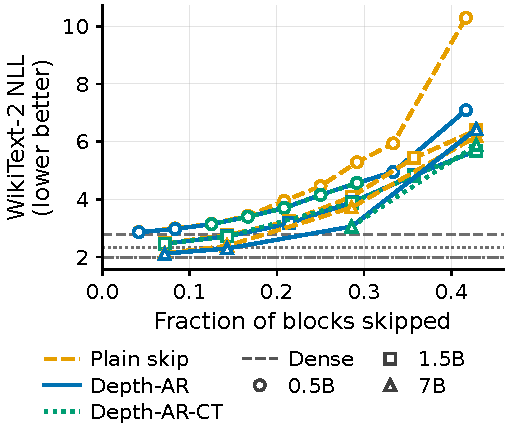
\includegraphics[width=\linewidth]{figures/fig2a_frontier.pdf}
\caption{The quality--compression frontier.}
\label{fig:frontier}
\end{subfigure}
\hfill
\begin{subfigure}{0.48\textwidth}
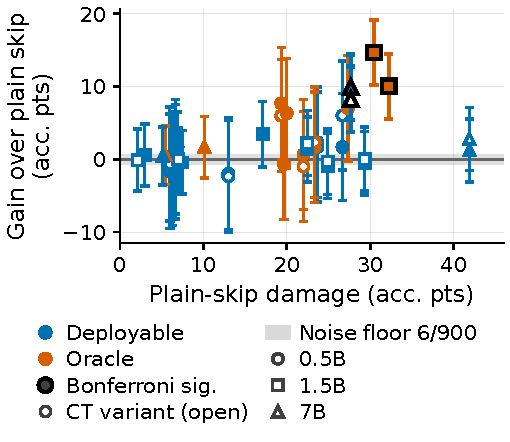
\includegraphics[width=\linewidth]{figures/fig2b_significant_gains.pdf}
\caption{Gain against damage.}
\label{fig:gains}
\end{subfigure}
\caption{\textbf{Prediction pays off in proportion to what skipping destroys.}
\emph{Left:} WikiText-2 NLL against the fraction of blocks skipped, for Qwen2.5-0.5B (circles),
1.5B (squares) and 7B (triangles), with layers chosen by measured residual damage and every
predictor skipping the identical blocks. \mname sits below plain skipping at every measured
fraction on 0.5B and 1.5B, and the cross-token variant sits below \mname; the dashed lines are
the dense models. \emph{Right:} every accuracy comparison in the paper, plotted as the gain over
plain skipping against the damage plain skipping does. Bars are $95\%$ confidence intervals; the
grey band is the measured reproducibility floor of the evaluation itself (6 answers of 900 in
BF16). Points cluster on zero where damage is small: at light budgets there is nothing to
recover. The four comparisons that survive Bonferroni correction across all 63 tests (filled)
all sit at the right, where skipping is destructive, and they are reached under both the
deployable damage-based rule and the recovery-maximising one. Hardware and protocol:
\Cref{sec:app-protocol}.}
\label{fig:gains-pair}
\end{figure*}
